\documentclass[letterpaper,17pt]{recipe}
\usepackage{graphicx}
\usepackage[spanish]{babel}
\usepackage{setspace}
\doublespacing
\setlength\parindent{0pt}
\setlength\parskip{2ex plus 0.5ex}

\begin{document}
\recipe{Camarones a la Diabla}
\begin{figure}[htpb]
	\centering
	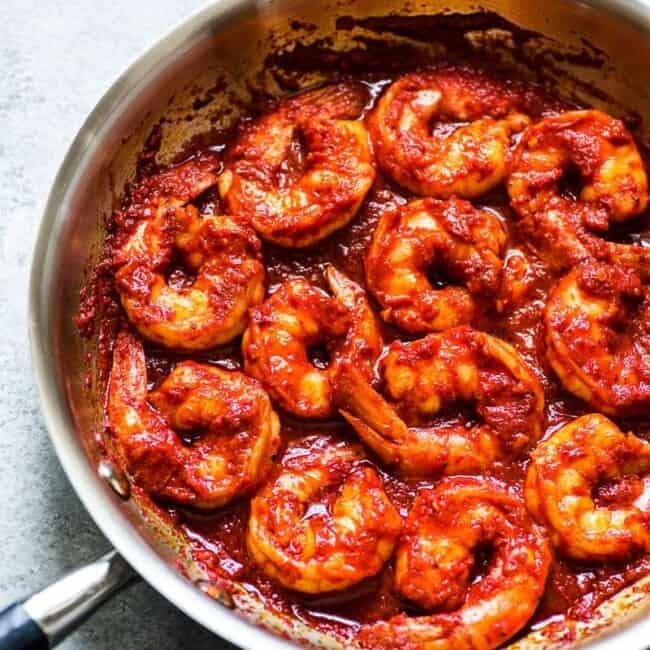
\includegraphics[width=0.4\textwidth]{shrimp.jpg}
	\caption{Los camarones a la Diabla (también conocidos como camarones diablo) son camarones grandes y jugosos cubiertos con una salsa de chile rojo brillante que están listos para comer en 30 minutos. (sin gluten, bajo en carbohidratos, paleo)}
	\label{fig:shrimp-jpg}
\end{figure}
\ingred{8 chiles guajillos, enjuagados, sin tallos ni semillas;\\
 	3 chiles de árbol, enjuagados y sin tallos;\\
	3 tomates roma, picados;\\
	2 dientes de ajo;\\
	1/2 cebolla blanca mediana, picada en trozos grandes;\\
	1 cucharadita de sal kosher;\\
	4 cucharadas de aceite de oliva;\\
	1,5 libras de camarones crudos grandes, pelados, desvenados y con la cola;\\
	sal y pimienta negra, al gusto}

\begin{enumerate}
	\item En un tazón o cacerola mediana, agrega los chiles guajillo y de árbol secos. Agrega agua muy caliente o hirviendo hasta que los chiles estén completamente sumergidos. Cubra con una tapa o un plato grande y déjelo reposar durante 15 minutos, hasta que los chiles se ablanden.
	\item Con una espumadera, transfiera los chiles ablandados a una licuadora grande. Agrega los tomates, el ajo, la cebolla y la sal. Haga puré hasta que esté completamente suave. Pruebe y sazone con más sal, si es necesario. Si la salsa está demasiado picante, agregue más tomates.
	\item Calienta una sartén o sartén grande a fuego medio-alto. Agrega el aceite de oliva y los camarones. Cocine los camarones durante 1 minuto por lado o hasta que estén de color rosa claro.
	\item Agregue la salsa de chile rojo a la sartén o sartén y mezcle para cubrir los camarones. Baje el fuego a medio y cocine de 3 a 5 minutos, hasta que la salsa esté burbujeante y caliente.
	\item Retira la sartén o sartén del fuego y sírvelo solo como aperitivo o con Auténtico Arroz Mexicano como comida.
\end{enumerate}
\end{document}
